\chapter{O problema dinâmico} 
\label{cap:3}

     
\section{Análise dinâmica de estruturas}

    \indent "Qualquer movimento que se repete em um determinado período é denominado vibração ou oscilação" (\citet{mechanicalvibrations2017}). A análise de vibrações é a área que se preocupa com os movimentos oscilatórios e com as forças a eles associadas em corpos sólidos, bem como com os efeitos mecânicos gerados no material devido a esses movimentos.  

\subsection{Conceitos Básicos} 

    \indent Em sistemas dinâmicos, tanto as variáveis de entrada quanto as de saída dependem do tempo e o movimento osciliatório é iniciado por uma excitação inicial. Um sistema vibratório é composto por mecanismos de armazenamento e dissipação de energia. Entre os mecanismos de armazenamento estão as energias cinética e potencial, enquanto a dissipação é representada pelo amortecimento do sistema dinâmico. A vibração do sistema ocorre devido à transferência alternada entre as energias cinética e potencial.\\
    \indent As classificações dos tipos de vibrações dependem da característica desse esforço e da resposta do sistema. Quando o sistema fica livre para vibrar por conta própria após um distúrbio, a vibração é classificada como livre, enquanto sistemas submetidos a forças externas são classificados como de vibração forçada. Em problemas de vibração forçada, caso a magnitude do esforço externo aplicado seja conhecida a todo instante, essa vibração é considerada determinística; caso contrário, é randômica. A dissipação de energia devido à presença de amortecimento no sistema divide a classificação da vibração em amortecida e não amortecida. O comportamento de um sistema dinâmico pode ser linear ou não linear. A definição de linearidade é importante, pois o princípio de superposição modal pode ser aplicado apenas a vibrações lineares. \\
    \indent Nos sistemas vibratórios, os graus de liberdade (gdl) do problema representam a quantidade mínima de coordenadas independentes necessárias para determinar as posições de todas as partes do sistema em qualquer instante de tempo (\citet{vibrationcontinuoussystems2006}). Os gdls podem ser apresentados tanto como coordenadas cartesianas (em problemas de deslocamento das massas dos elementos do sistema) quanto como coordenadas polares (em problemas torcionais). A escolha do sistema de coordenadas busca simplificar a solução do problema em estudo. As coordenadas necessárias para a descrição do movimento de um sistema constituem um conjunto de coordenadas generalizadas.\\
    \indent A análise de vibrações inicia-se com a modelagem do problema, considerando as características apresentadas pelo sistema dinâmico alvo, para então proceder ao desenvolvimento das equações diferenciais que o governam. Em problemas discretos, a energia potencial elástica e a rigidez do sistema são representadas por molas, e a energia cinética é representada pela massa ou inércia dos elementos. A representação de um sistema dinâmico é feita por meio de diagramas com molas, massas e amortecedores. Um diagrama massa-mola-amortecedor permite a visualização dos elementos que compõem o sistema Figura~\ref{fig:3.1}. A Figura~\ref{fig:3.1-a} apresenta um pórtico plano com massa concentrada onde tanto a rigidez quanto o amortecimento são equivalentes por pavimento e a Figura~\ref{fig:3.1-b} apresenta um diagrama massa mola equivalente ao pórtico. \\

     \begin{figure}[htbp]
        \centering
        \caption{Diagramas de representação de problemas dinâmicos}
        \begin{subfigure}[b]{0.45\textwidth}
            \centering
            \includegraphics[width=\textwidth]{figuras/capitulo_3/1-a.png}
            \label{fig:3.1-a}
        \end{subfigure}
        \hfill
        \begin{subfigure}[b]{0.45\textwidth}
            \centering
            \includegraphics[width=\textwidth]{figuras/capitulo_3/1-b.png}
            \label{fig:3.1-b}
        \end{subfigure}
        \label{fig:3.1}

        {\small \textbf{Fonte:} Elaborado pelo autor (2026).}
    \end{figure}    

    \indent Sistemas vibratórios podem possuir mais de um ponto de massa concentrada (Figura~\ref{fig:3.2}) e um sistema de múltiplos gdls pode ser considerado um sistema de massas pontuais conectadas por molas e amortecedores (\citet{vibrationcontinuoussystems2006}).  

    \begin{figure}[htbp]
        \centering
        \caption{Diagramas dinâmico para sistema aporticado de dois pavimentos.}
        \label{fig:3.2}
        \begin{subfigure}[b]{0.35\textwidth}
            \centering
            \includegraphics[width=\textwidth]{figuras/capitulo_3/2-a.png}
            \label{fig:3.2a}
        \end{subfigure}
        \hfill
        \begin{subfigure}[b]{0.6\textwidth}
            \centering
            \includegraphics[width=\textwidth]{figuras/capitulo_3/2-b.png}
            \label{fig:3.2b}
        \end{subfigure}

        {\small \textbf{Fonte:} Elaborado pelo autor (2026).}
    \end{figure}

    \indent Para os modelos dinâmicos, a massa — ou inércia — do sistema engloba os elementos capazes de ganhar ou perder energia cinética. Molas são elementos cuja massa e amortecimento são considerados nulos. São componentes que, quando submetidos a um esforço de tração, exercem uma força restauradora que tende a fazê-los retornar à sua configuração geométrica original (\citet{mechanicalvibrations2017}). A lei de Hooke estabelece que a força restauradora de uma mola é equivalente ao produto do coeficiente de elasticidade pelo deslocamento por ela sofrido: 

    \begin{equation}
        \mathbf{f} = k \mathbf{u}.
        \label{eq:3.1}
    \end{equation}

    \indent Nota-se que o coeficiente elástico é diretamente proporcional às forças aplicadas ao sistema; assim, a função da mola em sistemas dinâmicos é representar a rigidez do sistema frente aos esforços nele aplicados.  \\
    \indent Em problemas que envolvem rotação, é comum adotar o diagrama da Figura~\ref{fig:3.3}, no qual se utiliza a inércia em vez da massa dos elementos. 

    \begin{figure}[htbp]
        \centering
        \caption{Diagrama massa mola de problema torcional.}
        \includegraphics[width=\textwidth]{figuras/capitulo_3/3.png}
        \label{fig:3.3}

        {\small \textbf{Fonte:} Adaptado de \citet{mechanicalvibrations2017}}
    \end{figure}


    \indent Sistemas dinâmicos tendem a perder energia gradualmente na forma de calor ou som. A representação dessa perda de energia é feita por meio de amortecedores, que são elementos sem massa ou elasticidade, nos quais a força de amortecimento existe apenas se houver uma velocidade relativa entre as suas duas extremidades. Mesmo que o efeito do amortecimento seja pequeno, é importante considerá-lo para obter uma melhor exatidão na resposta do sistema aos esforços externos (\citet{mechanicalvibrations2017}). \\
    \indent Enquanto alguns sistemas apresentam uma representação simples, com as massas concentradas em determinados pontos, outros apresentam distribuição contínua de massa, elasticidade e amortecimento, principalmente em membros elásticos contínuos com um número infinito de gdl — como os modelos estudados neste trabalho. Os sistemas que apresentam massas concentradas (ou parâmetros agrupados) são chamados de modelos discretos, ao passo que aqueles com infinitos gdl são os sistemas contínuos. \\
    \indent Enquanto o movimento de um sistema discreto de $n$ gdl é governado por $n$ equações ordinárias de segunda ordem, os sistemas contínuos são governados por uma equação diferencial. A solução de equações diferenciais ordinárias é um processo mais simples, enquanto as equações diferenciais parciais são mais complexas de serem solucionadas e nem sempre apresentam solução em forma fechada. Todavia, as formas fechadas provêm maior discernimento quanto ao comportamento do sistema. Os métodos de solução para equações diferenciais parciais envolvem a discretização do domínio transformando a resolução do problema na solução de um sistema de equações algébricas. 

\section{Teoria da elasticidade e estado plano} 
	
    \indent A princípio, para descrever o comportamento de um material sob esforços, bem como as tensões e deformações internas que surgem, seria necessário considerar o movimento de seus átomos, quais são governados pela mecânica quântica. Entretanto, existem maneiras mais simples de modelar esse comportamento, como a mecânica do contínuo. A mecânica do contínuo ignora a discreticidade do mundo, tratando-o como um meio macroscópico observável (\citet{tadmor2012continuum}). 
	
    \subsection{Conceitos básicos de mecânica do contínuo e teoria da elasticidade}

    \indent Os corpos são formados por partículas e moléculas nas quais atuam forças moleculares que se opõem à mudança de forma. Conforme indica a terceira lei de Newton, a aplicação de forças externas resulta em forças reativas que tendem a impedir a alteração do corpo. O estado de deformação ocorre com a aplicação de forças externas, e as partículas deslocam-se continuamente até que o equilíbrio entre as forças exteriores e interiores seja estabelecido (\citet{resistenciadosmateriais1976}).  \\
    \indent Tensões são forças distribuídas em superfícies externas ou internas de um corpo. A função das tensões é servir como medida de intensidade de uma força, ou seja, representar a distribuição das forças sobre determinada área. A importância da análise de tensões reside no fato de que falhas mecânicas não estão diretamente relacionadas à força bruta exercida no objeto, mas sim à concentração dessas forças em determinadas superfícies. \\
    \indent Para a análise de um ponto no interior de um objeto sujeito a esforços concentrados e de superfície, realiza-se um corte em uma seção do sólido onde se encontra esse ponto. Os esforços internos encontram-se distribuídos e não são perfeitamente uniformes, normais ou tangenciais à superfície de corte (Figura~\ref{fig:3.6}); contudo, possuem componentes normais e tangenciais que simplificam a análise (esforços de tração ou compressão e cisalhamento). 

    \begin{figure}[htbp]
        \centering
        \caption{Sólido sob ação de forças pontuais e distribuídas.}
        \includegraphics[width=\textwidth]{figuras/capitulo_3/6.png}
        \label{fig:3.6}

        {\small \textbf{Fonte:} \citet{elasticitytheoryapplicationsnumerics2021}}
    \end{figure}

	\indent Ao considerar uma área infinitesimal $dA$ em um plano, utilizando um sistema de coordenadas cartesianas \(x_1\), \(x_2\) e \(x_3\) ao redor do ponto de interesse, as tensões resultantes de um esforço interno $F$ no elemento são calculadas por: 

    \begin{equation}
        \boldsymbol{\sigma}_{ij}  = \frac{dF_{i}}{dA_j}, 
        \label{eq:3.10}
    \end{equation}


	\indent As tensões normais à superfície de corte correspondem às tensões de compressão ou tração, enquanto as tensões tangenciais correspondem às tensões de cisalhamento. Para cada plano, em um sistema tridimensional, existem duas tensões de cisalhamento. Essas tensões são componentes da tensão de cisalhamento total, dada por: 

    \begin{equation}
        (\boldsymbol{\sigma}_{ij})_{\text{cis,res}} = \sqrt{ \sum_{j=1,\, j \neq i}^{3} \boldsymbol{\sigma}_{ij}^2 }.
        \label{eq:3.11}
    \end{equation}


    \indent Para um plano de corte, o vetor de tensões (vetor de tração) é a combinação linear dos componentes normais e tangenciais; desse modo, para um versor $\hat{\mathbf{e}}$, o vetor de tensões é descrito como: 

    \begin{equation}
        \mathbf{t} = t_j \,\hat{\mathbf{e}}_j .
        \label{eq:3.12}
    \end{equation}


\indent A descrição completa do estado de tensões em um ponto exigiria o conhecimento de infinitos planos de corte. Como a variedade de tensões ao redor de um ponto é infinita, descrevê-las acuradamente demandaria o uso de uma esfera infinitesimal. Todavia, graças ao método de transformação de coordenadas, basta conhecer as tensões em apenas três planos ortogonais para descrever o estado de tensões em qualquer superfície (\citet{roarksformulasstressstrainninthedition2020}). A combinação dos vetores de tensões nos três planos forma o tensor de tensões \(\boldsymbol{\sigma}\), cujas componentes, nos eixos coordenados, coincidem com as \(t_{ij}\):

    \begin{equation}
    \boldsymbol{\sigma} = \begin{bmatrix} 
        t_{11} & t_{12} & t_{13} \\ 
        t_{21} & t_{22} & t_{23} \\ 
        t_{31} & t_{32} & t_{33}  
    \end{bmatrix}.
    \label{eq:3.13}
    \end{equation}


\indent Enquanto o vetor de tensões se trata de uma força por unidade de área, o mesmo não pode ser dito do tensor de tensões isoladamente. Todavia, o tensor carrega as informações necessárias para a construção de qualquer vetor de tensões. Uma propriedade vital é o princípio de Cauchy, que afirma que o vetor tensão em qualquer ponto de uma superfície interna de um meio contínuo depende unicamente do vetor normal unitário: 

\begin{equation}
    t_i = \sigma_{ij} n_j \quad \text{ou} \quad \mathbf{t}^{(\hat{\mathbf{n}})} = \boldsymbol{\sigma} \cdot \hat{\mathbf{n}}.
    \label{eq:3.14}
\end{equation}

\indent Essa relação permite a construção de qualquer vetor de tensões por meio do tensor de tensões $\boldsymbol{\sigma}$ e do vetor normal unitário $\hat{\mathbf{n}}$ à superfície em questão. \\
\indent Em uma classe específica de problemas de elasticidade — seja pela geometria, propriedades do material, condições de contorno ou cargas externas —, a solução independe de uma das coordenadas. Esses problemas se enquadram na chamada elasticidade plana \citet{introductioncontinuummechanics2013}. Essa hipótese simplifica o cálculo, permitindo que um problema tridimensional seja tratado como bidimensional. Considerando nulas as tensões na direção \(x_3\) (Figura~\ref{fig:3.8}), chega-se à matriz: 

\begin{equation}
    \boldsymbol{\sigma} = \begin{bmatrix} 
        t_{11} & t_{12} \\ 
        t_{21} & t_{22}  
    \end{bmatrix} =
    \begin{bmatrix} 
        \sigma_{11} & \tau_{12} \\ 
        \tau_{21} & \sigma_{22}  
    \end{bmatrix}.
    \label{eq:3.15}
\end{equation}

  \begin{figure}[H]
        \centering
        \caption{Área infinitesimal sob ação de tensões normais e de cisalhamento.}
        \includegraphics[width=0.6\textwidth]{figuras/capitulo_3/8.png}
        \label{fig:3.8}

        {\small \textbf{Fonte:} Elaborado pelo autor (2026).}
    \end{figure}


\indent Os problemas de elasticidade plana são descritos por um conjunto de duas equações diferenciais acopladas, expressas em termos de duas variáveis dependentes que representam as componentes do vetor deslocamento. Eles dividem-se entre grandes e pequenas deformações. No regime de pequenas deformações, um sólido pode apresentar extensões ou deformações por cisalhamento. A Figura~\ref{fig:3.9} será utilizada no estudo da relação geométrica em um plano para a obtenção das componentes da deformação. 


\begin{figure}[H]
    \centering
    \caption{Elemento distorcido.}
    \resizebox{0.9\textwidth}{!}{\input{figuras/capitulo_3/figura}}
    \label{fig:3.9}

    {\small \textbf{Fonte:} Adaptado de (\citet{elasticitytheoryapplicationsnumerics2021})}
\end{figure}


\indent A deformação por alongamento (ou encurtamento) é a variação relativa ao comprimento inicial. Assumindo o valor de $u_1(x_1 + dx,x_2) \approx u_1(x_1,x_2) + (\partial u_1 / \partial x_1) dx_1$, a deformação no eixo $x_1$ é:

\begin{equation}
    \epsilon_{x_1} = \frac{A^{\prime}B^{\prime} - AB}{AB}
    \label{eq:3.16}
\end{equation}

\indent A distância $A^{\prime}B^{\prime}$ é:

\begin{equation}
    A^{\prime}B^{\prime} = \sqrt{\left( dx_1 + \frac{\partial u_1}{\partial x_1}dx_1 \right)^2 + \left( \frac{\partial u_2}{\partial x_1}dx_1 \right)^2} \approx \left( 1 + \frac{\partial u_1}{\partial x_1} \right) dx_1
    \label{eq:3.17}
\end{equation}

\indent Substituindo a Eq.~\ref{eq:3.17} na Eq.~\ref{eq:3.16}, a deformação no eixo $x_1$ resulta em: 

\begin{equation}
    \epsilon_{x_1} =  \frac{\partial u_1}{\partial x_1},
    \label{eq:3.18}
\end{equation}


\indent E, de maneira análoga, no eixo $x_2$: 

\begin{equation}
    \epsilon_{x_2} =  \frac{\partial u_2}{\partial x_2}.
    \label{eq:3.19}
\end{equation}


\indent A deformação por cisalhamento é definida como a mudança no ângulo de duas direções outrora ortogonais em um meio contínuo. Utilizando a Figura~\ref{fig:3.9}, a deformação é definida como: 

\begin{equation}
    2\epsilon_{x_1x_2} = \frac{\pi}{2} - \angle C^{\prime}A^{\prime}B^{\prime} = \alpha + \beta.
    \label{eq:3.20}
\end{equation}

\indent Em regime de pequenas deformações, os ângulos $\alpha$ e $\beta$ são suficientemente pequenos para que se possa aproximá-los por suas respectivas tangentes. Assim, a Eq.~\ref{eq:3.20} assume a forma

\begin{equation}
    2\varepsilon_{x_1x_2} = \frac{\dfrac{\partial u_2}{\partial x_1}\,dx_1}{dx_1 + \dfrac{\partial u_1}{\partial x_1}\,dx_1} + \frac{\dfrac{\partial u_1}{\partial x_2}\,dx_2}{dx_2 + \dfrac{\partial u_2}{\partial x_2}\,dx_2}.
    \label{eq:3.20b}
\end{equation}

\noindent Cada uma das frações pode ser reescrita de maneira mais conveniente:
\begin{equation*}
    \frac{\dfrac{\partial u_2}{\partial x_1}\,dx_1}{dx_1\bigl(1 + \tfrac{\partial u_1}{\partial x_1}\bigr)}
    = \frac{\partial u_2/\partial x_1}{1 + \partial u_1/\partial x_1},
    \qquad
    \frac{\dfrac{\partial u_1}{\partial x_2}\,dx_2}{dx_2\bigl(1 + \tfrac{\partial u_2}{\partial x_2}\bigr)}
    = \frac{\partial u_1/\partial x_2}{1 + \partial u_2/\partial x_2}.
\end{equation*}
Como as deformações são pequenas, os termos $\partial u_1/\partial x_1$ e $\partial u_2/\partial x_2$ são muito menores que a unidade. Utilizando a expansão em série de Taylor
$$\frac{1}{1+x} = 1 - x + \mathcal{O}(x^2), \qquad |x|\ll 1,$$ e desprezando os produtos de ordem superior, chega-se à expressão linearizada

\begin{equation}
    2\varepsilon_{x_1x_2} = \frac{\partial u_1}{\partial x_2} + \frac{\partial u_2}{\partial x_1}.
    \label{eq:3.21}
\end{equation}

\indent Em notação tensorial, as deformações são descritas como: 

\begin{equation}
    \boldsymbol{\varepsilon} = \frac{1}{2} \left( \nabla \mathbf{u} + (\nabla \mathbf{u})^T \right), \qquad \varepsilon_{ij} = \frac{1}{2} \left( \frac{\partial u_i}{\partial x_j} +  \frac{\partial u_j}{\partial x_i} \right).
    \label{eq:3.22}
\end{equation}

\indent De acordo com \citet{continuummechanicsengineers2010}, o comportamento elástico em um corpo é caracterizado por duas premissas: \\
\indent A tensão no material é uma função unívoca da deformação. O material possui a propriedade de retornar à sua geometria original após a remoção dos esforços aplicados. \\
\indent As leis constitutivas permitem relacionar as tensões com as deformações do material. Assume-se que cada componente de tensão se relaciona linearmente com os componentes de deformação, de modo que: 

\begin{equation}
    \boldsymbol{\sigma} = \mathbb{C} : \boldsymbol{\varepsilon}, \qquad \sigma_{ij} = \mathbb{C}_{ijkl} \varepsilon_{kl},
    \label{eq:3.23}
\end{equation}

\noindent onde $\mathbb{C}_{ijkl}$ é um tensor elástico de quarta ordem que contém todos os parâmetros necessários para caracterizar o material. \\
\indent Segundo \citet{introductioncontinuummechanics2013}, um material é dito isotrópico (modelo constitutivo de interesse neste trabalho) quando suas propriedades mecânicas podem ser descritas independentemente da direção; caso contrário, é anisotrópico. Ao tomar uma direção com base $e_i$, a relação constitutiva será igual à Eq.~\ref{eq:3.23}. Caso se analise uma direção $e_i^\prime$, a relação será: 

\begin{equation}
    \boldsymbol{\sigma}^\prime = \mathbb{C}^\prime : \boldsymbol{\varepsilon}^\prime, \qquad \sigma_{ij}^\prime = \mathbb{C}_{ijkl}^\prime \varepsilon_{kl}^\prime.
    \label{eq:3.24}
\end{equation}

\indent Em um modelo isotrópico, os tensores $\mathbb{C}_{ijkl}$ e $\mathbb{C}_{ijkl}^\prime$ devem ser idênticos, independentemente da base utilizada. Para um sólido elástico linear isotrópico, o tensor de elasticidade de quarta ordem admite a forma geral
\begin{equation}
    \mathbb{C}_{ijkl} = \lambda\,\delta_{ij}\delta_{kl} + \mu\bigl(\delta_{ik}\delta_{jl} + \delta_{il}\delta_{jk}\bigr),
    \label{eq:3.25}
\end{equation}
\noindent em que \(\lambda\) e \(\mu\) são os parâmetros de Lamé, relacionados ao módulo de Young \(E\) e ao coeficiente de Poisson \(\nu\) por
\begin{equation}
    \lambda = \frac{E\nu}{(1+\nu)(1-2\nu)}, \qquad
    \mu = \frac{E}{2(1+\nu)}.
    \label{eq:3.26}
\end{equation}
\noindent Equivalentemente, a relação constitutiva pode ser escrita de forma compacta como
\begin{equation}
    \boldsymbol{\sigma} = \lambda\,(\operatorname{tr}\boldsymbol{\varepsilon})\,\mathbf{I} + 2\mu\,\boldsymbol{\varepsilon}.
    \label{eq:3.27}
\end{equation}

\indent O tensor constitutivo de uma material isotrópico linear pode ser separado em duas parcelas, uma referente às componentes normais e outra as componentes tangenciais do tensor de deformações,
\begin{equation} 
    \mathbb{C} = \mathbb{C}_N + \mathbb{C}_S,
    \label{eq:3.a1}
\end{equation} 

\noindent tal que:

\begin{equation*}
    \begin{aligned}
        (\mathbb{C}_N)_{ijkl} = \lambda \delta_{ij} \delta_{kl} + \mu \delta_{ik} \delta_{jl} \\
        (\mathbb{C}_N)_{ijkl} = \mu \delta_{il} \delta_{jk}
    \end{aligned}
\end{equation*}

\indent Os problemas de estado plano são obtidos como reduções desse mesmo tensor. No estado plano de deformações (\(\varepsilon_{33}=\varepsilon_{13}=\varepsilon_{23}=0\)) e no estado plano de tensões (\(\sigma_{33}=\sigma_{13}=\sigma_{23}=0\)), a relação constitutiva se reduz a duas dimensões, e as equações de equilíbrio e compatibilidade são ajustadas consoante as condições impostas.\\
\indent A tensão de von Mises, ou tensão efetiva, trata-se de um escalar que relaciona as componentes do tensor de tensões. Segundo \citet{elasticitytheoryapplicationsnumerics2021}, se em algum ponto a tensão de von Mises for igual à tensão de escoamento, então o material é considerado estar sob condição de falha. A tensão de von Mises, para o estado plano de tensões, é calculada por: 

\begin{equation}
    \sigma_{vM} = \sqrt{\frac{3}{2} \sigma_{ij}\sigma_{ij} - \frac{1}{2}(\sigma_{kk})^2}
    \label{eq:3.vm}
\end{equation}


\subsubsection{Notação de Voigt}

\indent Embora a notação tensorial seja a forma natural e mais compacta de descrever a mecânica do contínuo, em métodos numéricos (especialmente no Método dos Elementos Finitos e no Método dos Elementos Virtuais) é comum adotar a \emph{notação de Voigt}. Nessa representação, os tensores simétricos de segunda ordem (tensão e deformação) são reorganizados como vetores coluna de seis componentes (em 3D) ou três componentes (em 2D), e o tensor elástico de quarta ordem passa a ser representado por uma matriz simétrica.

\noindent Em três dimensões, a correspondência é
\begin{equation}
    \boldsymbol{\sigma}^{\text{V}} =
    \begin{Bmatrix}
        \sigma_{11} \\ \sigma_{22} \\ \sigma_{33} \\ \sigma_{23} \\ \sigma_{13} \\ \sigma_{12}
    \end{Bmatrix},
    \qquad
    \boldsymbol{\varepsilon}^{\text{V}} =
    \begin{Bmatrix}
        \varepsilon_{11} \\ \varepsilon_{22} \\ \varepsilon_{33} \\ 2\varepsilon_{23} \\ 2\varepsilon_{13} \\ 2\varepsilon_{12}
    \end{Bmatrix},
    \label{eq:3.28}
\end{equation}
em que o fator 2 que multiplica as componentes de cisalhamento da deformação (deformações de engenharia) garante que o produto interno seja preservado:
\begin{equation}
    \boldsymbol{\sigma}:\boldsymbol{\varepsilon} = (\boldsymbol{\sigma}^{\text{V}})^T \boldsymbol{\varepsilon}^{\text{V}}.
\end{equation}
A relação constitutiva \(\boldsymbol{\sigma} = \mathbb{C}:\boldsymbol{\varepsilon}\) torna-se, então,
\begin{equation}
    \boldsymbol{\sigma}^{\text{V}} = \mathbf{C}\,\boldsymbol{\varepsilon}^{\text{V}},
    \label{eq:3.29}
\end{equation}
onde \(\mathbf{C}\) é a matriz elástica \(6\times 6\) (em 3D) ou \(3\times 3\) (em 2D).

\noindent Para o material isotrópico linear, a matriz de Voigt em três dimensões lê-se
\begin{equation}
    \mathbf{C} =
    \begin{bmatrix}
        \lambda+2\mu & \lambda & \lambda & 0 & 0 & 0 \\
        \lambda & \lambda+2\mu & \lambda & 0 & 0 & 0 \\
        \lambda & \lambda & \lambda+2\mu & 0 & 0 & 0 \\
        0 & 0 & 0 & \mu & 0 & 0 \\
        0 & 0 & 0 & 0 & \mu & 0 \\
        0 & 0 & 0 & 0 & 0 & \mu
    \end{bmatrix}.
    \label{eq:3.30}
\end{equation}

\noindent No estado plano de deformações a matriz reduz-se a
\begin{equation}
    \mathbf{C}^{\text{pd}} =
    \frac{E}{(1+\nu)(1-2\nu)}
    \begin{bmatrix}
        1-\nu & \nu & 0 \\
        \nu & 1-\nu & 0 \\
        0 & 0 & \dfrac{1-2\nu}{2}
    \end{bmatrix},
    \label{eq:3.31}
\end{equation}
\noindent enquanto no estado plano de tensões obtém-se
\begin{equation}
    \mathbf{C}^{\text{pt}} =
    \frac{E}{1-\nu^2}
    \begin{bmatrix}
        1 & \nu & 0 \\
        \nu & 1 & 0 \\
        0 & 0 & \dfrac{1-\nu}{2}
    \end{bmatrix}.
    \label{eq:3.32}
\end{equation}

\indent A notação de Voigt será adotada, sempre que conveniente, nos capítulos seguintes, por ser a forma mais prática para a implementação computacional dos métodos discretos. A correspondência com a notação tensorial permanece unívoca e será utilizada sempre que for necessário enfatizar aspectos contínuos ou propriedades de invariância.

\subsection{Energia de deformação}

\indent A formulação da energia de deformação constitui uma consequência direta das relações constitutivas da elasticidade linear. Conforme apresentado por \citet{continuummechanicsengineers2010}, a energia de deformação por unidade de volume, denotada por $W$, pode ser definida a partir da função de energia elástica, de modo que o tensor de tensões seja obtido pela derivação dessa função em relação ao tensor de deformações. Para pequenas deformações, tem-se
\begin{equation}
    \sigma_{ij}=\frac{\partial W}{\partial \varepsilon_{ij}}.
    \label{eq:3.a2}
\end{equation}

\indent A existência de uma função de energia de deformação implica, ainda, a simetria maior do tensor constitutivo, consequentemente, a energia de deformação pode ser expressa como
\begin{equation}
    W=\frac{1}{2}\mathbb{C}_{ijkl}\varepsilon_{ij}\varepsilon_{kl}=\frac{1}{2}\sigma_{ij}\varepsilon_{ij}.
    \label{eq:3.a3}
\end{equation}

\noindent A mesma formulação mostra que a taxa de trabalho realizada pelas tensões é igual à taxa de variação da energia armazenada.\\
\indent Aplicando a separação do tensor constitutivo definido na equação~\ref{eq:3.a1} na equação~\ref{eq:3.a3}, chega-se à: $$W=\frac{1}{2}\left((\mathbb{C}_N)_{ijkl}+(\mathbb{C}_S)_{ijkl}\right)\varepsilon_{ij}\varepsilon_{kl} = $$
\begin{equation}
    W=\frac{1}{2}(\mathbb{C}_N)_{ijkl}\varepsilon_{ij}\varepsilon_{kl} + \frac{1}{2}(\mathbb{C}_S)_{ijkl}\varepsilon_{ij}\varepsilon_{kl}.
    \label{eq:3.a4}
\end{equation}

\indent O que implica que a energia de deformação pode ser dividida em uma parcela normal e outra de cisalhamento:
\begin{equation}
    W = W_N + W_S
    \label{eq:3.a5}
\end{equation}

\subsection{Formulação da equação governante}

\indent A segunda lei de Newton afirma que o somatório das forças em um sistema é equivalente à variação da quantidade de movimento; assim: 

\begin{equation}
    \frac{d}{dt} \left( m \frac{d\mathbf{u}(\mathbf{x},t)}{dt} \right) = \mathbf{F}.
    \label{eq:3.33}
\end{equation}


\indent Em problemas nos quais não há variação de massa, a Eq.~\ref{eq:3.33} simplifica-se para: 

\begin{equation}
    m \ddot{\mathbf{u}}(\mathbf{x},t) = \mathbf{F}.
    \label{eq:3.34}
\end{equation}


\indent Em materiais contínuos, a massa não é pontual; destarte, a Eq.~\ref{eq:3.34} torna-se: 

\begin{equation}
    d\mathbf{F} = dm \,\ddot{\mathbf{u}}(\mathbf{x},t)
    \label{eq:3.35}
\end{equation}


\indent A densidade $\rho$ representa a massa distribuída no volume do sólido. Em termos contínuos: 

\begin{equation}
    \rho = \frac{dm}{dV}
    \label{eq:3.36}
\end{equation}

\indent Substituindo a Eq.~\ref{eq:3.35} na Eq.~\ref{eq:3.36}, obtém-se a força de inércia: 

\begin{equation}
    d\mathbf{F} = \rho \,\ddot{\mathbf{u}}(\mathbf{x},t)\, dV \quad \therefore \quad \mathbf{F} = \int_V \rho \,\ddot{\mathbf{u}}(\mathbf{x},t)\, dV.
    \label{eq:3.37}
\end{equation}

\indent Os esforços mais comuns que atuam sobre um sólido são as forças de corpo $\mathbf{b}$, que atuam em todo o volume do elemento: 

\begin{equation}
    \mathbf{F}_{\text{corpo}} = \int_V \mathbf{b} \, dV,
    \label{eq:3.38}
\end{equation}

	
e os esforços de superfície, que se encontram distribuídos, independentemente de esse elemento fazer parte da superfície delimitadora externa ou ser um elemento arbitrário no interior do corpo \citet{continuummechanicsengineers2010}. As forças de superfície $\mathbf{t}^{(\hat{n})}$ possuem dimensões de força por unidade de área. A partir da Eq.~\ref{eq:3.10}, essas forças podem ser obtidas do produto do vetor de tensões normal superfície e um diferencial de superfície $dS$:
	
\begin{equation}
    \mathbf{F}_{\text{surf}} = \int_S \mathbf{t}^{(\hat{n})} \, dS.
    \label{eq:3.39}
\end{equation}


\indent O princípio de d'Alembert introduz uma força fictícia, denominada força de inércia, que permite que o equilíbrio dinâmico seja formulado com os mesmos conceitos do equilíbrio estático (\citet{introductionfiniteelementvibrationanalysis2010}) ou a segunda lei de Newton. Em um corpo sujeito a forças de corpo e de superfície, a equação de equilíbrio é a soma das Eq.~\ref{eq:3.38} e \ref{eq:3.39} igual à equação \ref{eq:3.37}, resultando em:

\begin{equation}
    \int_S \mathbf{t}^{(\hat{n})} \, dS + \int_V \mathbf{b} \, dV - \int_V \rho \ddot{\mathbf{u}}(\mathbf{x},t) \, dV = 0.
    \label{eq:3.40}
\end{equation}


\indent Aplicando o princípio de Cauchy a parcelo do vetor de tensões:

\begin{equation}
    \int_S \mathbf{t}^{(\hat{n})} \, dS = \int_S \boldsymbol{\sigma} \cdot \hat{\mathbf{n}} \, dS,
    \label{eq:3.41}
\end{equation}


e utilizando o teorema da divergência: 
 
\begin{equation}
    \int_S \boldsymbol{\sigma} \cdot \hat{\mathbf{n}} \, dS = \int_V \nabla \cdot \boldsymbol{\sigma} \, dV. 
    \label{eq:3.42}
\end{equation}


\indent Substituindo a Eq.~\ref{eq:3.42} na Eq.~\ref{eq:3.40}: 

\begin{equation}
    \int_V \nabla \cdot \boldsymbol{\sigma} \, dV  + \int_V \mathbf{b} \, dV - \int_V \rho \ddot{\mathbf{u}}(\mathbf{x},t) \, dV = 0.
    \label{eq:3.43}
\end{equation}

\indent Como todos os argumentos estão integrados em um diferencial de volume que é arbitrário, o integrando deve ser nulo em todos os pontos, obtendo-se a equação de movimento: 

\begin{equation}
    \nabla \cdot \boldsymbol{\sigma}  +  \mathbf{b}  = \rho \ddot{\mathbf{u}}(\mathbf{x},t).
    \label{eq:3.44}
\end{equation}


\subsubsection{As condições de solução de uma equação diferencial}

\indent Como destacam \citet{hillen2019partial}, uma equação diferencial parcial pode possuir uma infinidade de soluções, incluindo aproximações polinomiais de diversas ordens ou combinações de funções exponenciais e trigonométricas. Condições adicionais são indispensáveis para garantir a unicidade da solução, sendo elas as condições iniciais e as condições de contorno. As condições iniciais estão comumente atreladas ao domínio temporal, dadas em um instante inicial: 

\begin{equation}
    \mathbf{u}(\mathbf{x},t=0) = \mathbf{u}_0(\mathbf{x})
    \label{eq:3.45}
\end{equation}

	
\indent As condições de contorno são utilizadas para descrever o comportamento do sistema nas fronteiras espaciais do domínio. Dentre elas, destacam-se as condições de Dirichlet, Neumann e Robin. As restrições de Dirichlet impõem diretamente os valores da variável no contorno. Em uma fronteira $\partial \Omega$ com $\mathbf{x} \in \partial \Omega$, assumem a forma: 

\begin{equation}
    \mathbf{u}(\mathbf{x},t) = \mathbf{g}(\mathbf{x},t).
    \label{eq:3.46}
\end{equation}


\indent Já os problemas com condições de Neumann possuem a derivada normal externa especificada na fronteira: 

\begin{equation}
    \frac{\partial \mathbf{u}}{\partial n} = \mathbf{g},
    \label{eq:3.47}
\end{equation}
	
\noindent onde \(\partial\mathbf{u}/\partial n = (\nabla\mathbf{u})\cdot\mathbf{n}\) é a derivada direcional. \citet{farlow1993partial} ressalta que as condições de Neumann puras diferem das demais por permitirem infinitas soluções (movimentos de corpo rígido). Desse modo, exige-se pelo menos uma restrição adicional (como um ponto de Dirichlet) para encontrar uma solução particular. A condição de Robin, por sua vez, é uma composição linear das condições de Dirichlet e Neumann: 

\begin{equation}
    \alpha \mathbf{u} + \beta \frac{\partial \mathbf{u}}{\partial n} = \mathbf{g}.
    \label{eq:3.48}
\end{equation}

\indent Em problemas de mecânica estrutural, as condições de contorno estão diretamente atreladas aos vínculos ou apoios físicos. Regiões com movimento totalmente restrito configuram condições de Dirichlet, enquanto vínculos elásticos comportam-se como condições de Robin 

\section{Métodos aproximados} 

\indent As soluções aproximadas para equações diferenciais satisfazem o equilíbrio em um sentido médio, não pontualmente em todas as coordenadas. Tais aproximações são tipicamente expandidas como uma combinação linear de um conjunto de funções de base ponderadas por parâmetros arbitrários \citet{finlayson1972method}. 

\subsection{Métodos dos resíduos ponderados}

\indent Os métodos dos resíduos ponderados englobam técnicas para a obtenção de soluções aproximadas de equações diferenciais lineares ou não lineares, servindo também como pilar matemático fundamental para formulações variacionais empregadas no Método dos Elementos Finitos (MEF) e no Método dos Elementos Virtuais (MEV). 
\indent Dado um operador diferencial $L$ e um termo de excitação de forças ou fontes $F$, a função resíduo surge da diferença entre a aplicação do operador sobre a solução aproximada $u_h$ e o termo exato $F$:

\begin{equation}
    L(u_h) = F.
    \label{eq:3.49}
\end{equation}

\indent Nesse escopo, a solução candidata é expandida usando um conjunto predefinido de funções teste (funções de aproximação) $\varphi_i$, ponderadas por coeficientes ou graus de liberdade ajustáveis $a_i$ que garantem a melhor aproximação possível \citet{hughes1987finite}: 

\begin{equation}
    u_h(\mathbf{x}) = \sum_{i=1}^n a_i \varphi_i(\mathbf{x}).
    \label{eq:3.50}
\end{equation}


\indent O Método de Galerkin minimiza o resíduo da equação por intermédio da ortogonalização frente a um conjunto de funções peso $w_i$: 

\begin{equation}
    \int_{V} w_i (L(u_h) - F) \, dV = 0, \hspace{1cm} i = 1,2,...,n.
    \label{eq:3.51}
\end{equation}



\indent Essa abordagem ramifica-se em diversas variantes, distinguindo-se primordialmente pela escolha da função peso. As metodologias estão sintetizadas na Tabela~\ref{tab:3.2}:

    
\begin{table}[htbp]
    \centering
    \caption{Principais variações do método dos resíduos ponderados}
    \begin{tabular}{p{5cm}p{5cm}p{5cm}}
        \textbf{Método} & \textbf{Função peso ($w_i$)} & \textbf{Ideia principal} \\
        \hline
        \textbf{Colocação} & Delta de Dirac ($w = \delta(x_j - x)$) & Impõe ($R=0$) em pontos específicos do domínio. \\[3pt]
        \textbf{Subdomínios} & ($w_i=1$) em cada subdomínio e ($0$) fora & Anula o resíduo em média em cada subdomínio. \\[3pt]
        \textbf{Mínimos Quadrados} & ($w_i=\dfrac{\partial R}{\partial a_i}$) & Minimiza a norma quadrática do resíduo. \\[3pt]
        \textbf{Galerkin} & ($w_i=\varphi_i$) (mesmas funções de aproximação) & Utiliza as mesmas funções para aproximação e ponderação. \\[3pt]
        \textbf{Petrov–Galerkin} & ($w_i\neq \varphi_i$) & Utiliza funções de ponderação diferentes das funções de aproximação.
    \end{tabular}
    \label{tab:3.2}
\end{table}


\indent De acordo com \citet{rao2017finite}, a formulação de Galerkin destaca-se por fornecer resultados altamente robustos em mecânica dos sólidos. Trata-se, historicamente, do método mais recorrente para a derivação variacional das matrizes de elementos finitos. \\
\indent Resolver a equação diferencial no seu formato "forte" (original) requer um elevado grau de regularidade (continuidade) da função aproximadora. A variável primária necessita ser diferenciável até a ordem máxima estipulada pelo operador analítico. A migração para a forma fraca, de natureza integral, relaxa drasticamente essa exigência. 

\subsection{Forma fraca da equação governante}

\indent Resgatando a equação do movimento (Eq.~\ref{eq:3.44}), o resíduo $R$ exibe a seguinte forma: 

\begin{equation}
    R(\mathbf{u}, \ddot{\mathbf{u}}) = \nabla \cdot \boldsymbol{\sigma}  +  \mathbf{b}  -  \rho \ddot{\mathbf{u}}.
    \label{eq:3.52}
\end{equation}


\indent O método de Galerkin exige que o resíduo seja ortogonal à cinemática admissível, representada por uma função peso $\mathbf{w}$ genérica, ou seja: 

\begin{equation}
    \int_{V} \mathbf{w} \cdot \bigl( \nabla \cdot \boldsymbol{\sigma}  +  \mathbf{b}  -  \rho \ddot{\mathbf{u}} \bigr)\, dV = 0.
    \label{eq:3.53}
\end{equation}

\indent Aplicando a identidade $$\mathbf{w} \cdot (\nabla \cdot \boldsymbol{\sigma}) = \nabla \cdot (\boldsymbol{\sigma}^T \mathbf{w}) - \nabla\mathbf{w} : \boldsymbol{\sigma}$$ (ver, por exemplo, \citet{hughes1987finite}) e o teorema da divergência, obtém-se a forma fraca:

\begin{equation}
    \int_{V} \rho \, \mathbf{w} \cdot \ddot{\mathbf{u}} \, dV + \int_{V} \nabla\mathbf{w} : \boldsymbol{\sigma} \, dV  
    = \int_{V} \mathbf{w} \cdot \mathbf{b} \, dV + \int_{S} \mathbf{w} \cdot \mathbf{t}^{(\hat{n})} \, dS.
    \label{eq:3.54}
\end{equation}

\indent O gradiente do deslocamento virtual pode ser decomposto em sua parte simétrica (tensor de deformações) e antissimétrica (rotação rígida local): 

\begin{equation}
    \nabla\mathbf{w} = \boldsymbol{\varepsilon}(\mathbf{w}) + \boldsymbol{\omega}(\mathbf{w}).
    \label{eq:3.55}
\end{equation}

\indent Projetando-o sobre o tensor de tensões via produto interno de tensores (duplo produto escalar): 

\begin{equation}
    \nabla\mathbf{w} : \boldsymbol{\sigma}  = \bigl( \boldsymbol{\varepsilon}(\mathbf{w}) + \boldsymbol{\omega}(\mathbf{w}) \bigr) : \boldsymbol{\sigma}  = \boldsymbol{\varepsilon}(\mathbf{w}) : \boldsymbol{\sigma}  + \boldsymbol{\omega}(\mathbf{w}) : \boldsymbol{\sigma}.
    \label{eq:3.56}
\end{equation}

\indent Como o tensor de tensões $\boldsymbol{\sigma}$ é simétrico (equilíbrio de momento angular local) e a contração de um tensor simétrico com um antissimétrico é nula, reduz-se a:

\begin{equation}
    \nabla\mathbf{w} : \boldsymbol{\sigma}  =  \boldsymbol{\varepsilon}(\mathbf{w}) : \boldsymbol{\sigma} .
    \label{eq:3.57}
\end{equation}

\indent Substituindo na forma fraca (Eq.~\ref{eq:3.54}) e adotando a relação constitutiva elástica linear \(\boldsymbol{\sigma} = \mathbb{C} : \boldsymbol{\varepsilon}(\mathbf{u})\), obtém-se:

\begin{equation}
    \int_{V} \rho \, \mathbf{w} \cdot \ddot{\mathbf{u}} \, dV + \int_{V}  \boldsymbol{\varepsilon}(\mathbf{w}) : \mathbb{C} : \boldsymbol{\varepsilon}(\mathbf{u})  \, dV  
    = \int_{V} \mathbf{w} \cdot \mathbf{b} \, dV + \int_{S} \mathbf{w} \cdot \mathbf{t}^{(\hat{n})} \, dS.
    \label{eq:3.58}
\end{equation}

\indent Ao introduzir as funções de interpolação $\boldsymbol{\varphi}$, a forma discreta do problema resulta no sistema algébrico:

\begin{equation}
\begin{aligned}
    &\Bigl( \int_{\Omega} \rho \, \boldsymbol{\varphi}^T \boldsymbol{\varphi} \, d\Omega \Bigr) \ddot{\mathbf{u}} 
    + \Bigl( \int_{\Omega}  \boldsymbol{\varepsilon}(\boldsymbol{\varphi}) : \mathbb{C} : \boldsymbol{\varepsilon}(\boldsymbol{\varphi}) \, d\Omega \Bigr) \mathbf{u}   
    = \int_{\Omega} \boldsymbol{\varphi} \cdot \mathbf{b} \, d\Omega + \int_{\Gamma} \boldsymbol{\varphi} \cdot \mathbf{t}^{(\hat{n})} \, d\Gamma.
\end{aligned}
    \label{eq:3.59}
\end{equation}

\indent A representação matricial condensada deste arcabouço dá origem à equação fundamental da dinâmica estrutural computacional (sem amortecimento): 

\begin{equation}
    \mathbf{M} \ddot{\mathbf{u}} + \mathbf{K} \mathbf{u} = \mathbf{f}.
    \label{eq:3.60}
\end{equation}

\indent Uma escrita alternativa — muito popular em publicações matemáticas — utiliza o jargão de operadores bilineares para abstrair a forma fraca: 

\begin{equation}
    m(\ddot{\mathbf{u}}, \mathbf{w}) + a(\mathbf{u}, \mathbf{w}) =  ( \mathbf{f}, \mathbf{w} ) + (g_N,\mathbf{w})_{\Gamma_N}.
    \label{eq:3.61}
\end{equation}

\indent Os termos $a(\cdot,\cdot)$ e $(\cdot,\cdot)$ são exemplos de formas simétricas e bilineares. Uma forma é simétrica quando o valor da função é o mesmo para qualquer ordem dos argumentos: 
$$a(\mathbf{u},\mathbf{v}) = a(\mathbf{v},\mathbf{u}),$$ 
e bilinear quando linearidade em relação a cada uma de suas variáveis separadamente, mantendo a outra constante: 
$$a(c_1 \mathbf{u} + c_2 \mathbf{v}, \mathbf{w}) = c_1 a(\mathbf{u},\mathbf{w}) + c_2 a(\mathbf{v},\mathbf{w}).$$\\
\indent \citet{hughes1987finite} afirma que a notação utilizada na Eq.~\ref{eq:3.61} é concisa e captura aspectos matemáticos importantes. Devido a isso, essa notação será utilizada diversas vezes no decorrer dos próximos capítulos em definições.\\ 
\indent Os termos descritos na equação~\ref{eq:3.58} estão em função de um diferencial de volume. Como problemas de estado plano são bidimensionais, a seguinte transformação é aplicada ao diferencial:
\begin{equation*}
    dV = d(x,y) \, dA,
\end{equation*}
\noindent onde $dA$ é um diferencial de área e $d(x,y)$ a função relacionada a espessura do sólido. Para os casos em que $d(x,y)$ é constante, a equação~\ref{eq:3.58} se torna:
\begin{equation}
    d \int_{A} \rho \, \mathbf{w} \cdot \ddot{\mathbf{u}} \, dA + d \int_{A}  \boldsymbol{\varepsilon}(\mathbf{w}) : \mathbb{C} : \boldsymbol{\varepsilon}(\mathbf{u})  \, dA  
    = d\int_{A} \mathbf{w} \cdot \mathbf{b} \, dA + \int_{S} \mathbf{w} \cdot \mathbf{t}^{(\hat{n})} \, dS.  
    \label{3.58b}  
\end{equation}

\subsubsection{Formulação fraca da equação de vibração livre não amortecida}

\indent Segundo \citet{chopra2023dynamics}, uma estrutura é dita estar em estado de vibração livre quando perturbada de sua posição de equilíbrio estático e então permitida vibrar sem qualquer excitação dinâmica externa. Em sistemas de 1 gdl, a massa apresenta um deslocamento harmônico simples, como pode ser observado na Figura~\ref{fig:3.11}.

\begin{figure}[htbp]
    \centering
    \caption{Vibração livre de um sistema de um grau de liberdade.}
    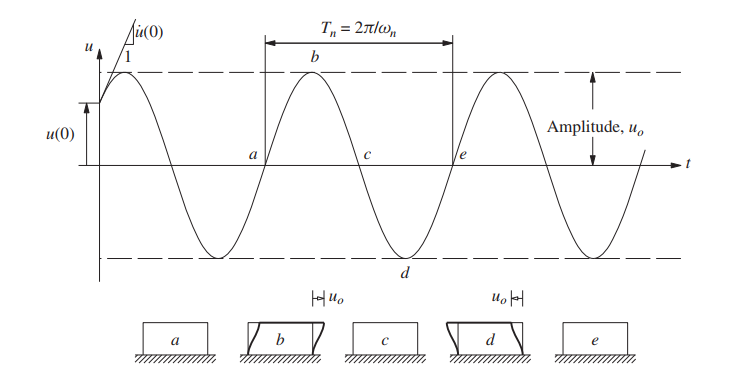
\includegraphics[width=\textwidth]{figuras/Capitulo_3/Captura de tela 2026-09-03 233659.png}
    \label{fig:3.11}
    {\small \textbf{Fonte:} \citet{chopra2023dynamics}}
\end{figure}

\indent Assim como pode ser observado na Figura~\ref{fig:3.11}, o tempo necessário para completar um ciclo de vibração livre é denominado período natural $T_n$, e a quantidade de ciclos por unidade de tempo é chamada de frequência natural $\omega_n$. A frequência natural depende das propriedades físicas do sistema, como massa e rigidez. \\
\indent Em problemas de múltiplos graus de liberdade, diferente do que ocorre em sistemas de 1 gdl, a vibração livre não é harmônica simples. A Figura~\ref{fig:3.12} ilustra o comportamento de um sistema com 2 gdls, no qual cada gdl apresenta uma frequência natural diferente. \\

\begin{figure}[htbp]
        \centering
        \caption{Resposta em vibração livre de um sistema de dois graus de liberdade.}
        \label{fig:3.12}
        \begin{subfigure}[b]{0.45\textwidth}
            \centering
            \includegraphics[width=\textwidth]{figuras/capitulo_3/f1.png}
            \label{fig:3.12a}
        \end{subfigure}
        \hfill
        \begin{subfigure}[b]{0.45\textwidth}
            \centering
            \includegraphics[width=\textwidth]{figuras/capitulo_3/f2.png}
            \label{fig:3.12b}
        \end{subfigure}

        {\small \textbf{Fonte:} \citet{chopra2023dynamics}}
    \end{figure}

\indent \citet{chopra2023dynamics} afirma que sob apropriada distribuição dos deslocamentos entre os graus de liberdade o sistema vibraria em movimento harmônico simples, como ilustrado na Figura~\ref{fig:3.4}. Cada uma dessas distribuições de deslocamentos é denominada modo de vibração natural. Os modos de vibração podem ser definidos como formas de vibrar, ou padrões de vibração, quando aplicados a um sistema com diversos pontos que apresentam diferentes amplitudes e deflexões (\citet{braun2001encyclopedia}). A frequência associada a cada modo é chamada de frequência natural modal. 

 \begin{figure}[htbp]
        \centering
        \caption{Modos de vibração de um sistema de dois graus de liberdade.}
        \label{fig:3.4}
        \begin{subfigure}[b]{0.45\textwidth}
            \centering
            \phantomcaption
            \includegraphics[width=\textwidth]{figuras/capitulo_3/4-a.png}
            \label{fig:3.4a}
        \end{subfigure}
        \hfill
        \begin{subfigure}[b]{0.45\textwidth}
            \centering
            \phantomcaption
            \includegraphics[width=\textwidth]{figuras/capitulo_3/4-b.png}
            \label{fig:3.4b}
        \end{subfigure}

        {\small \textbf{Fonte:} \citet{chopra2023dynamics}}
    \end{figure}


\indent Em sistemas contínuos são infinitos os modos de vibração de uma estrutura. Em contrapartida, em sistemas discretos, cada gdl corresponde a um possível deslocamento da estrutura, então, é perceptível que a quantidade de modos de vibração estão diretamente relacionadas à quantidade de gdls. Como se observa na Figura~\ref{fig:3.4b}, existe um ponto, chamado de nó, onde o deslocamento é sempre nulo. Cada modo de vibração possui um nó a mais que o anterior, até chegar ao último modo, no qual a quantidade de nós será igual à quantidade de gdls menos um. \\
\indent Em problemas lineares, os modos de vibração são independentes uns dos outros, o que significa que a vibração em um modo não influencia a vibração em outro. Cada modo de vibração possui uma forma modal específica descrita por um vetor de forma, denominado vetor modal \(\boldsymbol{\phi}_n\) e um valor escalar denominado coordenada modal \(q_n(t)\) que dita a amplitude do movimento conforme o tempo. Os deslocamentos de cada modo de vibração \(n\) são:

\begin{equation}
    \mathbf{u}_n(t) = \boldsymbol{\phi}_n \, q_n(t).
    \label{eq:3.62}
\end{equation}

\indent A solução da equação diferencial de um problema de vibração livre não amortecida de um sistema de um gdl é conhecida, tratando da equação de movimento harmônico simples; desse modo, $q(t)$ é especificado utilizando dois parâmetros escalares, $A$ e $B$, quais são determinados pelas condições de contorno iniciais do problema: 

\begin{equation}
    q_n(t) = A_n \cos{(\omega_n t)} + B_n \sin{(\omega_n t)}.
    \label{eq:3.63}
\end{equation}

\indent Unindo as Eq.~\ref{eq:3.62} e Eq.~\ref{eq:3.63}, chega-se à função dos deslocamentos modelada como um movimento harmônico:

\begin{equation}
    \mathbf{u}_n(\mathbf{x},t) = \boldsymbol{\phi}_n(\mathbf{x})\bigl(A_n \cos{(\omega_n t)} + B_n \sin{(\omega_n t)}\bigr).
    \label{eq:3.64}
\end{equation}

\indent Resgatando a equação de movimento (Eq.~\ref{eq:3.60}) e considerando que não há forças externas atuando sobre o sistema, obtém-se a equação de vibração livre não amortecida:

\begin{equation}
    \mathbf{M}\ddot{\mathbf{u}} + \mathbf{K}\mathbf{u}= \mathbf{0}.
    \label{eq:3.65}
\end{equation}

\indent Os valores de $\mathbf{u}$ e $\ddot{\mathbf{u}}$ como visto anteriormente podem ser descritos como uma combinação linear de modos de vibração, então, ao substituir a Eq.~\ref{eq:3.64} na Eq.~\ref{eq:3.65}, obtém-se:

\begin{equation}
    \bigl(\mathbf{K}\boldsymbol{\phi}_n -  \omega_n^2 \mathbf{M}\boldsymbol{\phi}_n\bigr) q_n(t) = \mathbf{0}.
    \label{eq:3.66}
\end{equation}

\indent Essa equação contém a solução trivial $\boldsymbol{q}_n(t) = \mathbf{0}$, que implica a não existência de movimento. Portanto, a obtenção das frequências naturais e dos modos de vibração provém da solução do problema de autovalor generalizado:

\begin{equation}
    \bigl(\mathbf{K} -  \omega_n^2 \mathbf{M}\bigr)\boldsymbol{\phi}_n = \mathbf{0}.
    \label{eq:3.67}
\end{equation}

\indent Segundo \citet{chopra2023dynamics}, quando $\omega_n \neq \omega_r$ a seguinte condição de ortogonalidade é satisfeita:

\begin{equation}
    \boldsymbol{\phi}_n^T \mathbf{K} \boldsymbol{\phi}_r = 0 \qquad \text{e} \qquad \boldsymbol{\phi}_n^T \mathbf{M} \boldsymbol{\phi}_r = 0.
    \label{eq:3.68}
\end{equation}

\indent Devido à independência dos modos de vibração, os deslocamentos de um sistema com múltiplos graus de liberdade pode ser descrita como uma combinação linear de seus modos de vibração (Figura~\ref{fig:3.5}), também conhecido como princípio da superposição modal:

\begin{equation}
    \mathbf{u} = \sum_{r=1}^{N} \boldsymbol{\phi}_r q_r.
    \label{eq:3.69}
\end{equation}

\begin{figure}[htbp]
    \centering
    \caption{Deslocamento de um pilar equivalente à soma dos deslocamentos de seus modos de vibração}
    \includegraphics[width=\textwidth]{figuras/capitulo_3/5.png}
    \label{fig:3.5}

    {\small \textbf{Fonte:} \citet{computingpropertiesdisplacementresponsemultidegreefreedomstructuresdifferentcircumstances2023}}
\end{figure}


    \indent As coordenadas modais são obtidas da relação:

    \begin{equation}
        q_n = \frac{\boldsymbol{\phi}_n^T \mathbf{M} \mathbf{u}}{\boldsymbol{\phi}_n^T \mathbf{M} \boldsymbol{\phi}_n}.
            \label{eq:3.70}
    \end{equation}



\subsection{Método de Galerkin com discretização do domínio}

\indent Métodos numéricos tais como o MEF e o MEV utilizam a mesma estrutura que o método de Galerkin. Contudo, esses métodos subdividem o domínio em subdomínios chamados elementos e aplicam em cada elemento a formulação fraca, obtida do método dos resíduos ponderados.\\
\indent Os métodos com discretização do domínio buscam encontrar a solução de um problema complexo ao substituí-lo por um problema mais simples. Nesses métodos, divide-se a região de solução (o domínio) em sub-regiões menores interconectadas, chamadas de elementos. Os elementos são conectados entre si por meio de juntas denominadas nós ou pontos nodais. Como as variações das variáveis de campo no contínuo são desconhecidas, assume-se que a solução pode ser aproximada por funções simples, as quais são escritas em função do valor das variáveis de campo nos nós \citet{rao2017finite}. O problema torna-se, então, solucionar um sistema linear de equações cujas incógnitas são as variáveis de campo nodais.\\
\indent Esses métodos, mesmo sendo aproximados, apresentam a vantagem de a solução ser aprimorada com o aumento do poder computacional — prática chamada de refino. Existem tipos principais de métodos de refino, que podem ser aplicados em conjunto. O refino $h$, por meio da redução do tamanho dos elementos, aumenta a quantidade deles no objeto de análise. O refino $p$ aumenta a ordem das funções de aproximação. O refino $r$ melhora a solução ao mover os nós para regiões de alto erro, sem que haja aumento no número de nós ou elementos. Em alguns casos, pode ser necessário refazer a distribuição de elementos na malha. Destaca-se em \citet{rao2017finite} que, mesmo com o refino $h$, existe um limite em que a solução para de se aproximar da solução analítica da equação diferencial Figura~\ref{fig:3.10}.

\begin{figure}[H]
    \centering
    \caption{Convergência da solução pelo método dos elementos finitos.}
    \resizebox{\textwidth}{!}{\begin{tikzpicture}[
    >={Stealth[length=2.5pt, width=1.8pt]},
    font=\scriptsize
]

    % --- EIXOS ---
    \draw[->] (0,0) -- (6,0) node[right, align=left] {Número de\\elementos};
    \draw[->] (0,0) -- (0,4);

    % --- LINHA TRACEJADA SUPERIOR (Exact solution) ---
    \draw[dashed, gray!80] (0,3) -- (5.5,3);
    \node[left, align=right] at (0,3) {Exata\\solução};

    % --- CURVA DE SOLUÇÃO (FEM) ---
    % Sintaxe corrigida usando plot smooth em vez de controls
    \draw[thick] plot [smooth, tension=0.7] coordinates {(0.5, 1.2) (2.0, 2.3) (3.5, 2.58) (4.5, 2.6)} -- (5.5, 2.6);

    % Ponto N0
    \fill (4.5, 2.6) circle (1.8pt);

    % Projeção tracejada para N0
    \draw[dashed, gray!80] (4.5, 0) -- (4.5, 2.6);
    \node[below] at (4.5,0) {$N_0$};

    % --- SETA E RÓTULO APONTANDO PARA A CURVA ---
    \node[anchor=north west, align=left] (labelfem) at (4.6, 2.3) {Solução dada pelo\\Método dos Elementos Finitos};
    % Referência corrigida sem espaços internos
    \draw[->] (labelfem.north west) -- (4.2, 2.58);

    % --- TEXTO INFERIOR ---
    \node[below=12pt] at (3,0) {Sem melhoria significativa além de $N_0$};

\end{tikzpicture}}
    \label{fig:3.10}    
    
    {\small \textbf{Fonte:} Adaptado de (\citet{rao2017finite})}
\end{figure}

\indent O processo de solução desses métodos envolve uma sequência de etapas fixas, sendo elas:

\begin{enumerate}
    \item Discretização do domínio do problema em uma malha de elementos;
    \item Adota-se uma interpolação adequada para o problema. A equação de aproximação deve ser simples do ponto de vista computacional e satisfazer certos requisitos de convergência;
    \item Derivam-se as matrizes e vetores elementares, tais quais as matrizes de rigidez e de massa, e os vetores de carga, seja utilizando um princípio variacional apropriado, através do método dos resíduos ponderados ou baseando-se em condições de equilíbrio;
    \item Unir as equações elementares em um sistema de equações global, como exemplo: $$\mathbf{K} = \bigcup_{e=1}^{n_{el}} \mathbf{k}_e \quad \text{(montagem)} $$
    \item Solucionar o sistema de equações para obtenção das variáveis de campo, e
    \item Computar outras variáveis através das variáveis de campo obtidas.
\end{enumerate}

\indent Os desenvolvimentos teóricos apresentados neste capítulo — desde a equação do movimento até a forma fraca e a análise modal — estabelecem as bases necessárias para a resolução numérica de problemas dinâmicos. A passagem da formulação contínua para a formulação discreta, no entanto, ainda depende da escolha do método numérico a ser aplicado. Contudo, a discretização de domínios com geometria irregular por meio de elementos finitos convencionais frequentemente exige malhas sofisticadas e restrições na escolha dos elementos. O Método dos Elementos Virtuais contorna parte dessas dificuldades ao admitir elementos de forma arbitrária, mantendo a consistência e a estabilidade da formulação. O Capítulo 4 é dedicado à apresentação dos fundamentos do MEV e à sua aplicação em problemas de dinâmica estrutural.